\documentclass[conference]{IEEEtran}
\usepackage[spanish, activeacute]{babel}
\usepackage[utf8]{inputenc}
\usepackage{amsmath, amssymb}
\usepackage{graphicx}
\usepackage{anysize}
\usepackage{hyperref}
\usepackage{caption}
\usepackage[table]{xcolor}
\usepackage{booktabs}

\usepackage{color}
\newcommand{\todo}{\textcolor{red}{TO DO:}\textcolor{blue}}

\title{}
\author{
\IEEEauthorblockN{
	Mauricio Solar \IEEEauthorrefmark{1}, Jonathan Antognini \IEEEauthorrefmark{1}, Marcelo Mendoza \IEEEauthorrefmark{1}, Jose Marroquín \IEEEauthorrefmark{1}, Cristián Maureira \IEEEauthorrefmark{1} \\
	Jorge Ibsen \IEEEauthorrefmark{2}, Lars Nyman \IEEEauthorrefmark{2}, 
	Eduardo Vera \IEEEauthorrefmark{3}, Diego Mardones \IEEEauthorrefmark{3}, Guillermo Cabrera \IEEEauthorrefmark{3},\\
	Paola Arellano \IEEEauthorrefmark{4},
	Karim Pichara \IEEEauthorrefmark{5}, Nelson Padilla \IEEEauthorrefmark{5},
	Ricardo Contreras \IEEEauthorrefmark{6}, \\ Neil Nagar \IEEEauthorrefmark{6},
	Victor Parada \IEEEauthorrefmark{7}.
}

\\

\IEEEauthorblockA{\IEEEauthorrefmark{1} Universidad Técnica Federico Santa María, Valparaiso, Chile}
\IEEEauthorblockA{\IEEEauthorrefmark{2} Atacama Large Millimeter/submillimeter Array, San Pedro de Atacama, Chile}		
\IEEEauthorblockA{\IEEEauthorrefmark{3} Universidad de Chile, Santiago, Chile}							
\IEEEauthorblockA{\IEEEauthorrefmark{4} Red Universitaria Nacional, Santiago, Chile}						
\IEEEauthorblockA{\IEEEauthorrefmark{5} Universidad Católica de Chile, Santiago, Chile}					
\IEEEauthorblockA{\IEEEauthorrefmark{6} Universidad de Concepción, Concepción, Chile}					
\IEEEauthorblockA{\IEEEauthorrefmark{7} Universidad de Santiago de Chile, Santiago, Chile}
}

\begin{document}

\maketitle

\begin{abstract}
\end{abstract}

\begin{IEEEkeywords}
\end{IEEEkeywords}

\section{Estado del Arte}

Desde el año 2002, proyectos de Observatorios Virtuales (VO's, por sus siglas en inglés) comenzaron a integrar
la Alianza Internacional de Observatorio Virtual bajo el \textbf{Guidelines
for Participation\footnote{La documentación se puede
encontrar en \url{http://www.ivoa.net/documents/latest/IVOAParticipation.html}}}.

Esos proyectos fueron fundados bajo programas privados y gubernamentales nacionales e
internacionales en colaboración con centro de estudios científicos,
universidades y otros. Quienes integran este proyecto, el Observatorio Virtual, 
comparten conocimientos entre ellos y la comunidad de modo estandarizado. Son 
ellos mismos quienes desarrollan estos estándares para el intercambio de 
información e interoperabilidad.

La Tabla \ref{table:integrantes} muestra los miembros de IVOA hasta mayo de
2013.

\begin{table}[h!t]
	\centering
	\caption{Integrantes de IVOA}	
	\begin{tabular}{l} \hline
		%\hline
		\textbf{Proyecto} \\\hline
			Argentina Virtual Observatory \cite{arg} \\
			Armenian Virtual Observatory \cite{arm}\\
			AstroGrid \cite{astrogrid}\\
			Australian Virtual Observatory \cite{aus}\\
			Brazilian Virtual Observatory \cite{bra}\\
			Canadian Virtual Observatory \cite{can}\\
			Chinese Virtual Observatory \cite{china}\\
			European Space Agency \cite{esa}\\
			European Virtual Observatory \cite{euro}\\
			German Astrophysical Virtual Observatory \cite{ger}\\
			Hungarian Virtual Observatory \cite{hun}\\
			Italian Virtual Observatory \cite{ita}\\
			Japanese Virtual Observatory \cite{jap}\\
			Observatorie Virtual France \cite{fra}\\
			Russian Virtual Observatory \cite{rus}\\
			Spanish Virtual Observatory \cite{spa}\\
			Ukranian Virtual Observatory \cite{ukr}\\
			Virtual Astronomical Observatory \cite{usa}\\
			Virtual Observatory India \cite{ind}\\
            \hline
	\end{tabular}
	\label{table:integrantes}
\end{table}

Casi la mitad de los observatorios virtuales de IVOA están en Europa: 9 del
total; 1 pertenece a Oceanía, 4 a América y 5 de ellos a Asia \footnote{Como la
mayor parte de Rusia está en territorio asiático, es considerado como uno de
los VO's de ese continente.} La figura 1 muestra la distribución de los
miembros de IVOA por continente.
	\begin{figure}[h!t]
		\begin{center}
			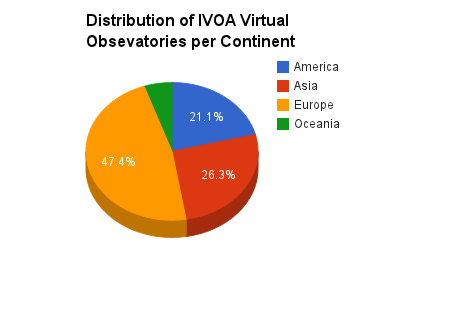
\includegraphics[width=0.5\textwidth]{img/ivoa_vos_distribution.png}
			\caption{Distribución por continente de IVOA.}
		\end{center}
	\end{figure}

Si Chile se convirtiera en miembro de IVOA, la distribución de los miembros
por continentes sería la que se muestra en la figura 2.
	\begin{figure}[h!t]
		\begin{center}
			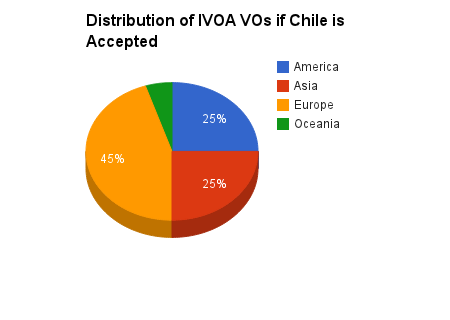
\includegraphics[width=0.5\textwidth]{img/if_chile_is_accepted.png}
			\caption{Distribución por continente incluyendo a Chile en IVOA.}
		\end{center}
	\end{figure}

Sin considerar el estado de los proyectos internos de los VO's, 
la membresía de Chile contribuiría a que América, llegue a la misma
cantidad en número de VO's que Asia. Por otra parte, este
hecho sería muy significativo, ya que un gran número de centros astronómicos
como los observatorios se instalan en este país. Por ahora, se pretende
trabajar con datos del proyecto ALMA. Actualmente se está realizando
un estudio de proyectos individuales que está ejecutando cada VO, sus resultados actuales
y los esperados.

\section{What has been done?}

\section{¿Qué se hará?}

Se van a testear los toolkits recomendados por IVOA: OpenCADC, SAADA, DaCHS,
DALServer. los cuales en su mayoría soportan TAP, SIA, SSA, SCS.

\section{¿Qué se ha hecho?}

Hasta el momento se han estudiado los estándares y protocolos de IVOA
necesarios para saber como trabajar con cada toolkits: Simple Image Access,
Simple Cone Search, Simple Spectra Access, Table Access Protocol, Observation
Data Model Core Components and its Implementation in the Table Access Protocol
\cite{obscore}, entre otros.

Además se han configurado las etapas iniciales de los toolkits: openCADC,
SAADA, DaCHS.

\section{Resultados esperados}

Se construirá a partir de estos toolkits un web service con el mismo modelo de
datos y la misma base datos, buscando ver cual es más escalable, estable, fácil
de manejar; además de cual tiene mejor documentación, y si es que tienen código
abierto, qué mejoras se podrían hacer. Se espera que la curva de aprendizaje de
uso de este tipo de toolkits comience con una pendiente bastante baja, esto
porque es necesario conocer algunos lenguajes de programación desde el punto de
vista práctico más que teórico, es decir, hay que lidiar con varias
bibliotecas, etc. Sin embargo se cree que una vez superada una etapa inicial la
curva de tome una pendiente más alta y finalmente decaiga.

\section{Expected Results}


%\section{Referencias}
%\bibliographystyle{plain}
%\bibliography{es_vo_sota}

\end{document}
